% Options for packages loaded elsewhere
\PassOptionsToPackage{unicode}{hyperref}
\PassOptionsToPackage{hyphens}{url}
%
\documentclass[
]{article}
\usepackage{amsmath,amssymb}
\usepackage{iftex}
\ifPDFTeX
  \usepackage[T1]{fontenc}
  \usepackage[utf8]{inputenc}
  \usepackage{textcomp} % provide euro and other symbols
\else % if luatex or xetex
  \usepackage{unicode-math} % this also loads fontspec
  \defaultfontfeatures{Scale=MatchLowercase}
  \defaultfontfeatures[\rmfamily]{Ligatures=TeX,Scale=1}
\fi
\usepackage{lmodern}
\ifPDFTeX\else
  % xetex/luatex font selection
\fi
% Use upquote if available, for straight quotes in verbatim environments
\IfFileExists{upquote.sty}{\usepackage{upquote}}{}
\IfFileExists{microtype.sty}{% use microtype if available
  \usepackage[]{microtype}
  \UseMicrotypeSet[protrusion]{basicmath} % disable protrusion for tt fonts
}{}
\makeatletter
\@ifundefined{KOMAClassName}{% if non-KOMA class
  \IfFileExists{parskip.sty}{%
    \usepackage{parskip}
  }{% else
    \setlength{\parindent}{0pt}
    \setlength{\parskip}{6pt plus 2pt minus 1pt}}
}{% if KOMA class
  \KOMAoptions{parskip=half}}
\makeatother
\usepackage{xcolor}
\usepackage[margin=1in]{geometry}
\usepackage{color}
\usepackage{fancyvrb}
\newcommand{\VerbBar}{|}
\newcommand{\VERB}{\Verb[commandchars=\\\{\}]}
\DefineVerbatimEnvironment{Highlighting}{Verbatim}{commandchars=\\\{\}}
% Add ',fontsize=\small' for more characters per line
\usepackage{framed}
\definecolor{shadecolor}{RGB}{248,248,248}
\newenvironment{Shaded}{\begin{snugshade}}{\end{snugshade}}
\newcommand{\AlertTok}[1]{\textcolor[rgb]{0.94,0.16,0.16}{#1}}
\newcommand{\AnnotationTok}[1]{\textcolor[rgb]{0.56,0.35,0.01}{\textbf{\textit{#1}}}}
\newcommand{\AttributeTok}[1]{\textcolor[rgb]{0.13,0.29,0.53}{#1}}
\newcommand{\BaseNTok}[1]{\textcolor[rgb]{0.00,0.00,0.81}{#1}}
\newcommand{\BuiltInTok}[1]{#1}
\newcommand{\CharTok}[1]{\textcolor[rgb]{0.31,0.60,0.02}{#1}}
\newcommand{\CommentTok}[1]{\textcolor[rgb]{0.56,0.35,0.01}{\textit{#1}}}
\newcommand{\CommentVarTok}[1]{\textcolor[rgb]{0.56,0.35,0.01}{\textbf{\textit{#1}}}}
\newcommand{\ConstantTok}[1]{\textcolor[rgb]{0.56,0.35,0.01}{#1}}
\newcommand{\ControlFlowTok}[1]{\textcolor[rgb]{0.13,0.29,0.53}{\textbf{#1}}}
\newcommand{\DataTypeTok}[1]{\textcolor[rgb]{0.13,0.29,0.53}{#1}}
\newcommand{\DecValTok}[1]{\textcolor[rgb]{0.00,0.00,0.81}{#1}}
\newcommand{\DocumentationTok}[1]{\textcolor[rgb]{0.56,0.35,0.01}{\textbf{\textit{#1}}}}
\newcommand{\ErrorTok}[1]{\textcolor[rgb]{0.64,0.00,0.00}{\textbf{#1}}}
\newcommand{\ExtensionTok}[1]{#1}
\newcommand{\FloatTok}[1]{\textcolor[rgb]{0.00,0.00,0.81}{#1}}
\newcommand{\FunctionTok}[1]{\textcolor[rgb]{0.13,0.29,0.53}{\textbf{#1}}}
\newcommand{\ImportTok}[1]{#1}
\newcommand{\InformationTok}[1]{\textcolor[rgb]{0.56,0.35,0.01}{\textbf{\textit{#1}}}}
\newcommand{\KeywordTok}[1]{\textcolor[rgb]{0.13,0.29,0.53}{\textbf{#1}}}
\newcommand{\NormalTok}[1]{#1}
\newcommand{\OperatorTok}[1]{\textcolor[rgb]{0.81,0.36,0.00}{\textbf{#1}}}
\newcommand{\OtherTok}[1]{\textcolor[rgb]{0.56,0.35,0.01}{#1}}
\newcommand{\PreprocessorTok}[1]{\textcolor[rgb]{0.56,0.35,0.01}{\textit{#1}}}
\newcommand{\RegionMarkerTok}[1]{#1}
\newcommand{\SpecialCharTok}[1]{\textcolor[rgb]{0.81,0.36,0.00}{\textbf{#1}}}
\newcommand{\SpecialStringTok}[1]{\textcolor[rgb]{0.31,0.60,0.02}{#1}}
\newcommand{\StringTok}[1]{\textcolor[rgb]{0.31,0.60,0.02}{#1}}
\newcommand{\VariableTok}[1]{\textcolor[rgb]{0.00,0.00,0.00}{#1}}
\newcommand{\VerbatimStringTok}[1]{\textcolor[rgb]{0.31,0.60,0.02}{#1}}
\newcommand{\WarningTok}[1]{\textcolor[rgb]{0.56,0.35,0.01}{\textbf{\textit{#1}}}}
\usepackage{graphicx}
\makeatletter
\def\maxwidth{\ifdim\Gin@nat@width>\linewidth\linewidth\else\Gin@nat@width\fi}
\def\maxheight{\ifdim\Gin@nat@height>\textheight\textheight\else\Gin@nat@height\fi}
\makeatother
% Scale images if necessary, so that they will not overflow the page
% margins by default, and it is still possible to overwrite the defaults
% using explicit options in \includegraphics[width, height, ...]{}
\setkeys{Gin}{width=\maxwidth,height=\maxheight,keepaspectratio}
% Set default figure placement to htbp
\makeatletter
\def\fps@figure{htbp}
\makeatother
\setlength{\emergencystretch}{3em} % prevent overfull lines
\providecommand{\tightlist}{%
  \setlength{\itemsep}{0pt}\setlength{\parskip}{0pt}}
\setcounter{secnumdepth}{-\maxdimen} % remove section numbering
\ifLuaTeX
  \usepackage{selnolig}  % disable illegal ligatures
\fi
\usepackage{bookmark}
\IfFileExists{xurl.sty}{\usepackage{xurl}}{} % add URL line breaks if available
\urlstyle{same}
\hypersetup{
  pdftitle={Replogle Miscalibration Exploration},
  pdfauthor={Gene},
  hidelinks,
  pdfcreator={LaTeX via pandoc}}

\title{Replogle Miscalibration Exploration}
\author{Gene}
\date{2025-06-23}

\begin{document}
\maketitle

This analysis explores our miscalibration issues with Replogle rd7 by
comparing to Velten's analysis.

\section{Sceptre Object Comparison}\label{sceptre-object-comparison}

Let's first compare our \texttt{sceptre\_object} to Velten's:

\begin{Shaded}
\begin{Highlighting}[]
\NormalTok{crispat\_sceptre\_object}
\end{Highlighting}
\end{Shaded}

\begin{verbatim}
## An object of class sceptre_object.
## 
## Attributes of the data:
##  • 17857 cells (17857 after cellwise QC)
##  • 36601 responses
##  • Low multiplicity-of-infection 
##  • 39 targeting gRNAs (distributed across 39 targets) 
##  • 113 non-targeting gRNAs 
##  • 11 covariates (Batch, cell, G2M_score, grna_n_nonzero, grna_n_umis, percent_mito, response_n_nonzero, response_n_umis, response_p_mito, S_score, total_UMI_counts)
\end{verbatim}

\begin{Shaded}
\begin{Highlighting}[]
\NormalTok{our\_sceptre\_object}
\end{Highlighting}
\end{Shaded}

\begin{verbatim}
## An object of class sceptre_object.
## 
## Attributes of the data:
##  • 616184 cells
##  • 36601 responses
##  • Low multiplicity-of-infection 
##  • 2536 targeting gRNAs (distributed across 2384 targets) 
##  • 130 non-targeting gRNAs 
##  • 6 covariates (batch, grna_n_nonzero, grna_n_umis, response_n_nonzero, response_n_umis, response_p_mito)
\end{verbatim}

The main differences are that

\begin{enumerate}
\def\labelenumi{\arabic{enumi}.}
\tightlist
\item
  they have way fewer cells,
\item
  they have 17 fewer NT gRNAs, and
\item
  they have extra covariates \texttt{G2M\_score} and \texttt{S\_score},
  which encode cell cycle state.
\end{enumerate}

The first is largely irrelevant to us because what we care about are the
cells with NT gRNAs only, and so we don't care about the other cells
anyways. An inspection of Velten's codebase revealed that they retained
all cells with NT gRNAs, \emph{except} those containing 17 NT gRNAs
found by Replogle to have apparent effects on genes. This brings us to
difference 2, which is very important. Throwing out NT gRNAs with an
apparent effect on genes prior to a calibration check is circular
reasoning, so we would want to repeat the calibration check with all NT
gRNAs. Item 3 may be important; if the cell cycle state acts as a
confounder. Let's check whether this is the case in the next section.

\section{Cell Cycle Effects on Non-targeting
gRNAs}\label{cell-cycle-effects-on-non-targeting-grnas}

Cell cycle state is known to impact gene expression; let's check based
on Velten's data whether it also impacts which gRNA a cell received.

\begin{Shaded}
\begin{Highlighting}[]
\FunctionTok{aov}\NormalTok{(S\_score }\SpecialCharTok{\textasciitilde{}}\NormalTok{ grna, }\AttributeTok{data =}\NormalTok{ velten\_df) }\SpecialCharTok{|\textgreater{}} \FunctionTok{summary}\NormalTok{()}
\end{Highlighting}
\end{Shaded}

\begin{verbatim}
##                Df Sum Sq Mean Sq F value   Pr(>F)    
## grna          112    5.4 0.04800   1.486 0.000695 ***
## Residuals   12611  407.4 0.03231                     
## ---
## Signif. codes:  0 '***' 0.001 '**' 0.01 '*' 0.05 '.' 0.1 ' ' 1
\end{verbatim}

\begin{Shaded}
\begin{Highlighting}[]
\FunctionTok{aov}\NormalTok{(G2M\_score }\SpecialCharTok{\textasciitilde{}}\NormalTok{ grna, }\AttributeTok{data =}\NormalTok{ velten\_df) }\SpecialCharTok{|\textgreater{}} \FunctionTok{summary}\NormalTok{()}
\end{Highlighting}
\end{Shaded}

\begin{verbatim}
##                Df Sum Sq Mean Sq F value  Pr(>F)   
## grna          112   22.1  0.1976   1.452 0.00134 **
## Residuals   12611 1716.2  0.1361                   
## ---
## Signif. codes:  0 '***' 0.001 '**' 0.01 '*' 0.05 '.' 0.1 ' ' 1
\end{verbatim}

We see that both cell cycle variables are correlated with gRNA, which
makes cell cycle a possible confounder. Maybe controlling for cell cycle
is enough to explain the miscalibration we're seeing.

\section{Calibration Check with Cell Cycle
Scores}\label{calibration-check-with-cell-cycle-scores}

We can't rely on the Velten data to get the cell cycle scores for our
calibration check, since they excluded 17 gRNAs. Therefore, I added
functionality to \texttt{ondisc} to calculate cell cycle during import
(which I hope will be independently useful). Below is a check that the
cell cycle scores I computed from scratch match those from the Velten
data, for the cells that overlap.

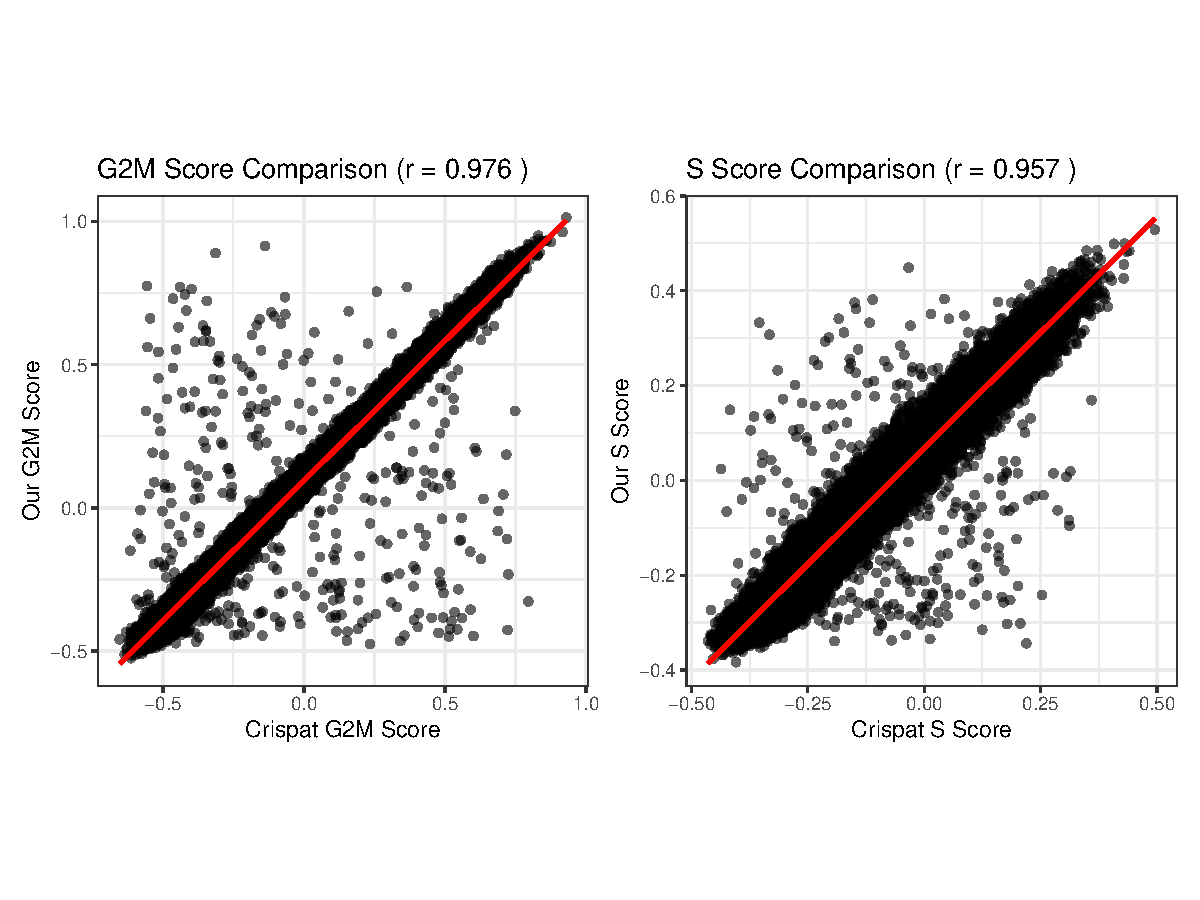
\includegraphics{replogle_miscalibration_exploration_files/figure-latex/cell-cycle-correlation-1.pdf}

The agreement seems pretty good. I then reran the calibration check
using this newly imported data on a million negative control pairs, with
the same formula (and other analysis parameters) used by Velten.

\includegraphics[width=1\linewidth]{../../../data/projects/sceptre3/replogle-2022/rd7-cell-cycle/plot_run_calibration_check}

Unfortunately, the miscalibration remains. Below is a table of how the
false positives are distributed across gRNAs:

\begin{verbatim}
## # A tibble: 49 x 2
##    grna_target                  n
##    <fct>                    <int>
##  1 non-targeting_vector_87     49
##  2 non-targeting_vector_59     21
##  3 non-targeting_vector_55     17
##  4 non-targeting_vector_63     14
##  5 non-targeting_vector_1       8
##  6 non-targeting_vector_112     8
##  7 non-targeting_vector_71      8
##  8 non-targeting_vector_34      6
##  9 non-targeting_vector_75      6
## 10 non-targeting_vector_106     4
## 11 non-targeting_vector_117     3
## 12 non-targeting_vector_13      2
## 13 non-targeting_vector_130     2
## 14 non-targeting_vector_16      2
## 15 non-targeting_vector_2       2
## 16 non-targeting_vector_28      2
## 17 non-targeting_vector_44      2
## 18 non-targeting_vector_47      2
## 19 non-targeting_vector_49      2
## 20 non-targeting_vector_61      2
## # i 29 more rows
\end{verbatim}

So we have about 20 NT gRNAs that make up the bulk of the problem;
likely these contain the 17 filtered out by Replogle and Velten.

\section{Conclusion}\label{conclusion}

Adding cell cycle didn't resolve the calibration issue, leading me to
believe that the Replogle data simply have NT gRNAs that ``didn't
work'', in the sense that they do have effects on some genes. In my
opinion, this means that the Replogle data are too low-quality for us to
analyze.

\end{document}
